\chapter{Ekler}
\section{Bir Oyuncak Kuram Icin Feynman Kurallari}
\begin{center}
\begin{figure}[!ph]
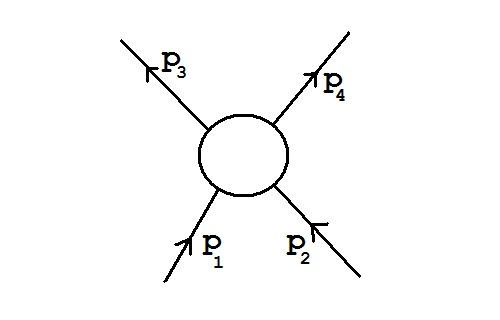
\includegraphics[scale=0.5]{feynmandiagram}
\caption{Dış çizgilerin etiketlendiği bir Feynman diagrami}
\end{figure}
\end{center}
Feynman diyagramına ait $\mathscr{M}$ genliğini bulmak icin Feynman kuralları.
\begin{enumerate}
\item \textbf{Notasyon :} Gelen ve çıkan dört-momentumları, $p_1,p_2,\cdots,p_n$ şeklinde iç momentumları, $q_1,q_2,\cdots$ şeklinde etiketleyin. Herbir çizginin yanında 'pozitif' yönü takip etmek için bir ok çizin (dış çizgiler için zamanda ileriye doğru, iç çizgiler için keyfi yönde).
\item \textbf{Köşe Faktörleri :} Her köşe için, bir
\begin{equation}
-ig
\end{equation}
faktöru yazın. $g$ \textit{çiftlenim sabiti} olarak adlandırılır. A, B, C arasındaki etkileşme şiddetini belirtir. Bu oyuncak kuramda $g$ momentum boyutundadır.
\item \textbf{Propagator :} Her bir çizgi için, bir
\begin{equation}
\frac{i}{q_j^2-m_j^2c^2}
\end{equation}
faktöru yazın. Burada $q_j$, çizginin dört-momentumunu ve $m_j$,çizgisinin betimlediği parçacığın kütlesidir.( $q_j\ neq  m_j^2c^2$ olduğuna dikkat edilmeli, çünkü sanal parçacık kütle kabuğu üzerinde değildir.)
\item \textbf{Enerji ve momentumun korunumu : } Her köşe için, aşağıdaki formda bir delta fonksiyonu yazın.
\begin{equation}
(2 \pi)^2 \delta^4(k_1+k_2+k_3)
\end{equation}
burada $k$'lar köşeye giren üç adet dört-momentumdur.(ok dışa doğru yönelmiş ise $k$ o çizginin dört-momentumunun eksi işaretlisidir). Bu faktör her köşede enerji ve momentum korunumunu zorunlu kılar, çünkü giren momentumların toplamı çıkan momentumlarının toplamına eşit değilse delta fonksiyonu sıfırdır.
\item \textbf{İç momentumlar üzerinde integral alma :} Her bir çizgi için aşağıdaki faktör yazılır.
\begin{equation}
\frac{1}{(2\pi)^4}d^4q_j
\end{equation}
ve tüm iç momentumlar üzerinden integral alınır.
\item \textbf{Delta fonksiyonunun iptali : } Sonuç ,
\begin{equation}
(2\pi)^4 \delta^4(p_1 +p_2+\cdots -p_n)
\end{equation}
şeklinde toplam enerji ve momentumun korunumunu yansıtan bir delta fonksiyonu içerir. Bu faktörü silip ve $i$ ile çarparsak,  sonuç.$\mathscr{M}$ yi verir.
\end{enumerate}
\section{MadGraph5 Kurulumu}
MadGraph\footnote{http://madgraph.phys.ucl.ac.be/} indirildikten sonra;
\begin{enumerate}
\item Sıkıştırılmıştır durumdan çıkartırılır.
\item Çıkartılan dosyanın içerisine terminalden girilir;\\
cd MG5\_ v\_****
\item  Gerekli programlar kurulur \\
MG5\_ aMC $>$ install pythia-pgs \\
MG5\_ aMC $>$ install ExRootAnalysis \\
MG5\_ aMC $>$ install MadAnalysis \\
MG5\_ aMC $>$ install Delphes 
\item Kurulumlar bittikten sonra MadGraph ile olay üretimine baslayabilirsiniz.
\end{enumerate}
\section{Olay Uretimi}
\subsection{Server Uzerinde Olay Uretimi}
Olaylarımızı server üzerinde gerçeklestirirken Shell Script kullandık. Bu bizim için kolaylık sağlamasının yanında zaman kazandırdı. İlgili Shell-script dosyası;

\begin{lstlisting}[language=bash,caption={Feynman diyagramlari ciziliyor}]
#!/bin/bash
echo "====================================="
echo "Start time   : `date`"
echo "====================================="
mg5=~/MG5_aMC_v2_3_3
myfilename="100-250 250-500 500-1000 1000-2500 2500-4000 4000-6000 6000-Inf"
min=(100 250 500 1000 2500 4000 6000)
max=(250 500 1000 2500 4000 6000 100000)
counter=0
for say in $myfilename
do
	cd ${mg5}
	sed -i '/output [a-z]*/c\output '"$say"'' ${mg5}/proc_card.dat
	cd ${mg5}
	./bin/mg5_aMC proc_card.dat
	sed -i '/ 0.0   = htjmin ! minimum jet HT=Sum(jet pt)/c\ '${min[$counter]}'   = htjmin ! minimum jet HT=Sum(jet pt)' ${mg5}/$say/Cards/run_card.dat
	sed -i '/ -1.0  = htjmax ! maximum jet HT=Sum(jet pt)/c\ '${max[$counter]}'   = htjmax ! maximum jet HT=Sum(jet pt)' ${mg5}/$say/Cards/run_card.dat
	sed -i '/ 0.0   = htjmin ! minimum jet HT=Sum(jet pt)/c\ '${min[$counter]}'   = htjmin ! minimum jet HT=Sum(jet pt)' ${mg5}/$say/Cards/run_card_default.dat
	sed -i '/ -1.0  = htjmax ! maximum jet HT=Sum(jet pt)/c\ '${max[$counter]}'   = htjmax ! maximum jet HT=Sum(jet pt)' ${mg5}/$say/Cards/run_card_default.dat
	counter=$((counter+1))
done
cd $mg5
./subrun1.sh
\end{lstlisting}
Burada olay Feynman diyagramlarını çizdiriyoruz. HT\footnote{Enerjisi}' sini istediğimiz aralıklarda tanımlayarak output dosyalarımızı HT aralıklarına göre alıyoruz.

\begin{lstlisting}[language=bash,caption={olay sayisi ayarlaniyor}]
#!/bin/bash

echo "====================================="
echo "Start time   : `date`"
echo "====================================="

#########################################

mg5=~/v2_3_0/MG5_aMC_v2_3_3
myfilename="100-250 250-500 500-1000 1000-2500 2500-4000 4000-6000 6000-Inf"
for say in $myfilename
do
sed -i '/  10000 = nevents ! Number of unweighted events requested/c\  100000 = nevents ! Number of unweighted events requested' ${mg5}/$say/Cards/run_card.dat
sed -i '/  10000 = nevents ! Number of unweighted events requested/c\  100000 = nevents ! Number of unweighted events requested' ${mg5}/$say/Cards/run_card_default.dat
done
cd $mg5
./subrun2.sh
exit 0
\end{lstlisting}
Burada olay sayısını 10000 den 100000 e ayarlıyoruz.

\begin{lstlisting}[language=bash,caption={olaylar uretiliyor}]
#!/bin/bash
mg5=~/MG5_aMC_v2_3_3
myfilename="100-250 250-500 500-1000 1000-2500 2500-4000 4000-6000 6000-Inf"
num_event=5
for say in $myfilename
do
cd ${mg5}/$say
./bin/madevent multi_run $num_event -f --laststep=pythia
done
exit 0
\end{lstlisting}

Artık son olarak Feynman diyagramlarını verdiğimiz olaya göre hesaplandırılması yapılıyor.

\begin{lstlisting}[language=bash,caption={dedektor similasyonu yapiliyor}]
#!/bin/bash
durmusmg5=/home/dyilmaz/tezAnaliz/analiz_1_pp_jj_jjj_jjjj/data
delphes=/home/dyilmaz/v2_3_0/MG5_aMC_v2_3_3/Delphes
HTbins="100-250 250-500 500-1000 1000-2500 2500-4000 4000-6000 6000-Inf"
	for ht in $HTbins # loop over all HTbin directories
	do
		mkdir $delphes/roots_for_$ht
		cd $durmusmg5/$ht/Events 
		for (( i=0 ; i < 5 ; ++i)) ;
		do
			cd run_01_$i
			gunzip tag_1_pythia_events.hep.gz # unzipping the generated hep files
			cd ..
		done
		cd $delphes
		for (( i=0 ; i < 5 ; ++i)) ;
		do
		./DelphesSTDHEP \
			$delphes/cards/delphes_card_CMS.tcl \
			$delphes/roots_for_$ht/run_01_$i.root \
			$durmusmg5/$ht/Events/run_01_$i/tag_1_pythia_events.hep 		done
		cd $delphes/roots_for_$ht
		hadd combined_$ht.root run_01_*.root
	done
exit 0

\end{lstlisting}

Burada hesaplanan Feynman diyagramları ve elde etmiş olduğumuz .hep\footnote{High Energy Physics} uzantılı dosyaları sıkıştırılmış halden çıkartıp delphes\_card\_CMS.tcl kartını kullanarak dedektor similasyonuna sokuyoruz. Bu işlemin sonucunda ürettiğimiz olaylar ROOT programında analiz etmek icin hazır hale geliyor.
\section{Olay Uretiminde kullanilan Kartlar} 
\begin{enumerate}


\item \textbf{proc\_card.dat}

\begin{lstlisting}
#************************************************************
#*                     MadGraph5_aMC@NLO                    *
#*                                                          *
#*                *                       *                 *
#*                  *        * *        *                   *
#*                    * * * * 5 * * * *                     *
#*                  *        * *        *                   *
#*                *                       *                 *
#*                                                          *
#*                                                          *
#*         VERSION 2.2.2                 2014-11-06         *
#*                                                          *
#*    The MadGraph5_aMC@NLO Development Team - Find us at   *
#*    https://server06.fynu.ucl.ac.be/projects/madgraph     *
#*                                                          *
#************************************************************
#*                                                          *
#*               Command File for MadGraph5_aMC@NLO         *
#*                                                          *
#*     run as ./bin/mg5_aMC  filename                       *
#*                                                          *
#************************************************************
set group_subprocesses Auto
set ignore_six_quark_processes False
set gauge unitary
set complex_mass_scheme False
import model sm-no_b_mass
define p = g u c d s u~ c~ d~ s~
define j = g u c d s u~ c~ d~ s~
define l+ = e+ mu+
define l- = e- mu-
define vl = ve vm vt
define vl~ = ve~ vm~ vt~
define p = u c s d b u~ c~ s~ d~ b~ g
define j = u c s d b u~ c~ s~ d~ b~ g
define l = e+ e- mu+ mu- ta+ ta-
generate p p > j j @0
add process p p > j j j @1
add process p p > j j j j @2
output 6000-Inf
\end{lstlisting}
\item \textbf{param\_card.dat}
\begin{lstlisting}
######################################################################
## PARAM_CARD AUTOMATICALY GENERATED BY MG5 FOLLOWING UFO MODEL   ####
######################################################################
##                                                                  ##
##  Width set on Auto will be computed following the information    ##
##        present in the decay.py files of the model.               ##
##        See  arXiv:1402.1178 for more details.                    ##
##                                                                  ##
######################################################################

###################################
## INFORMATION FOR MASS
###################################
Block mass 
    6 1.730000e+02 # MT 
   15 1.777000e+00 # MTA 
   23 9.118800e+01 # MZ 
   25 1.250000e+02 # MH 
## Dependent parameters, given by model restrictions.
## Those values should be edited following the 
## analytical expression. MG5 ignores those values 
## but they are important for interfacing the output of MG5
## to external program such as Pythia.
  1 0.000000 # d : 0.0 
  2 0.000000 # u : 0.0 
  3 0.000000 # s : 0.0 
  4 0.000000 # c : 0.0 
  5 0.000000 # b : 0.0 
  11 0.000000 # e- : 0.0 
  12 0.000000 # ve : 0.0 
  13 0.000000 # mu- : 0.0 
  14 0.000000 # vm : 0.0 
  16 0.000000 # vt : 0.0 
  21 0.000000 # g : 0.0 
  22 0.000000 # a : 0.0 
  24 80.419002 # w+ : cmath.sqrt(MZ__exp__2/2. + cmath.sqrt(MZ__exp__4/4. - (aEW*cmath.pi*MZ__exp__2)/(Gf*sqrt__2))) 

###################################
## INFORMATION FOR SMINPUTS
###################################
Block sminputs 
    1 1.325070e+02 # aEWM1 
    2 1.166390e-05 # Gf 
    3 1.180000e-01 # aS 

###################################
## INFORMATION FOR YUKAWA
###################################
Block yukawa 
    6 1.730000e+02 # ymt 
   15 1.777000e+00 # ymtau 

###################################
## INFORMATION FOR DECAY
###################################
DECAY   6 1.491500e+00 # WT 
DECAY  23 2.441404e+00 # WZ 
DECAY  24 2.047600e+00 # WW 
DECAY  25 6.382339e-03 # WH 
## Dependent parameters, given by model restrictions.
## Those values should be edited following the 
## analytical expression. MG5 ignores those values 
## but they are important for interfacing the output of MG5
## to external program such as Pythia.
DECAY  1 0.000000 # d : 0.0 
DECAY  2 0.000000 # u : 0.0 
DECAY  3 0.000000 # s : 0.0 
DECAY  4 0.000000 # c : 0.0 
DECAY  5 0.000000 # b : 0.0 
DECAY  11 0.000000 # e- : 0.0 
DECAY  12 0.000000 # ve : 0.0 
DECAY  13 0.000000 # mu- : 0.0 
DECAY  14 0.000000 # vm : 0.0 
DECAY  15 0.000000 # ta- : 0.0 
DECAY  16 0.000000 # vt : 0.0 
DECAY  21 0.000000 # g : 0.0 
DECAY  22 0.000000 # a : 0.0 
\end{lstlisting}
\item \textbf{run\_card.dat}
\begin{lstlisting}
#*********************************************************************
#                       MadGraph5_aMC@NLO                            *
#                                                                    *
#                     run_card.dat MadEvent                          *
#                                                                    *
#  This file is used to set the parameters of the run.               *
#                                                                    *
#  Some notation/conventions:                                        *
#                                                                    *
#   Lines starting with a '# ' are info or comments                  *
#                                                                    *
#   mind the format:   value    = variable     ! comment             *
#*********************************************************************
#
#*******************                                                 
# Running parameters
#*******************                                                 
#                                                                    
#*********************************************************************
# Tag name for the run (one word)                                    *
#*********************************************************************
  tag_1     = run_tag ! name of the run 
#*********************************************************************
# Run to generate the grid pack                                      *
#*********************************************************************
  False     = gridpack  !True = setting up the grid pack
#*********************************************************************
# Number of events and rnd seed                                      *
# Warning: Do not generate more than 1M events in a single run       *
# If you want to run Pythia, avoid more than 50k events in a run.    *
#*********************************************************************
  100000 = nevents ! Number of unweighted events requested
  0   = iseed   ! rnd seed (0=assigned automatically=default))
#*********************************************************************
# Collider type and energy                                           *
# lpp: 0=No PDF, 1=proton, -1=antiproton, 2=photon from proton,      *
#                                         3=photon from electron     *
#*********************************************************************
     1        = lpp1    ! beam 1 type 
     1        = lpp2    ! beam 2 type
     6500.0     = ebeam1  ! beam 1 total energy in GeV
     6500.0     = ebeam2  ! beam 2 total energy in GeV
#*********************************************************************
# Beam polarization from -100 (left-handed) to 100 (right-handed)    *
#*********************************************************************
     0.0     = polbeam1 ! beam polarization for beam 1
     0.0     = polbeam2 ! beam polarization for beam 2
#*********************************************************************
# PDF CHOICE: this automatically fixes also alpha_s and its evol.    *
#*********************************************************************
     nn23lo1    = pdlabel     ! PDF set                                     
     230000    = lhaid     ! if pdlabel=lhapdf, this is the lhapdf number
#*********************************************************************
# Renormalization and factorization scales                           *
#*********************************************************************
 False = fixed_ren_scale  ! if .true. use fixed ren scale
 False        = fixed_fac_scale  ! if .true. use fixed fac scale
 91.188  = scale            ! fixed ren scale
 91.188  = dsqrt_q2fact1    ! fixed fact scale for pdf1
 91.188  = dsqrt_q2fact2    ! fixed fact scale for pdf2
 -1 = dynamical_scale_choice ! Choose one of the preselected dynamical choices
 1.0  = scalefact        ! scale factor for event-by-event scales
#*********************************************************************
# Time of flight information. (-1 means not run)
#*********************************************************************
 -1.0 = time_of_flight ! threshold below which info is not written
#*********************************************************************
# Matching - Warning! ickkw > 1 is still beta
#*********************************************************************
 1 = ickkw            ! 0 no matching, 1 MLM, 2 CKKW matching
 1 = highestmult      ! for ickkw=2, highest mult group
 1 = ktscheme         ! for ickkw=1, 1 Durham kT, 2 Pythia pTE
 1.0 = alpsfact         ! scale factor for QCD emission vx
 False = chcluster        ! cluster only according to channel diag
 True = pdfwgt           ! for ickkw=1, perform pdf reweighting
 5 = asrwgtflavor     ! highest quark flavor for a_s reweight
 True = clusinfo         ! include clustering tag in output
 3.0 = lhe_version       ! Change the way clustering information pass to shower.        
#*********************************************************************
#**********************************************************
#
#**********************************************************
# Automatic ptj and mjj cuts if xqcut > 0
# (turn off for VBF and single top processes)
#**********************************************************
   True  = auto_ptj_mjj  ! Automatic setting of ptj and mjj
#**********************************************************
#                                                                    
#**********************************
# BW cutoff (M+/-bwcutoff*Gamma)
#**********************************
  15.0  = bwcutoff      ! (M+/-bwcutoff*Gamma)
#**********************************************************
# Apply pt/E/eta/dr/mij/kt_durham cuts on decay products or not
# (note that etmiss/ptll/ptheavy/ht/sorted cuts always apply)
#*************************************************************
   False  = cut_decays    ! Cut decay products 
#*************************************************************
# Number of helicities to sum per event (0 = all helicities)
# 0 gives more stable result, but longer run time (needed for
# long decay chains e.g.).
# Use >=2 if most helicities contribute, e.g. pure QCD.
#*************************************************************
   0  = nhel          ! Number of helicities used per event
#*******************                                                 
# Standard Cuts
#*******************                                                 
#                                                                    
#*********************************************************************
# Minimum and maximum pt's (for max, -1 means no cut)                *
#*********************************************************************
 20.0  = ptj       ! minimum pt for the jets 
 0.0  = ptb       ! minimum pt for the b 
 10.0  = pta       ! minimum pt for the photons 
 10.0  = ptl       ! minimum pt for the charged leptons 
 0.0  = misset    ! minimum missing Et (sum of neutrino's momenta)
 0.0  = ptheavy   ! minimum pt for one heavy final state
 -1.0  = ptjmax    ! maximum pt for the jets
 -1.0  = ptbmax    ! maximum pt for the b
 -1.0  = ptamax    ! maximum pt for the photons
 -1.0  = ptlmax    ! maximum pt for the charged leptons
 -1.0  = missetmax ! maximum missing Et (sum of neutrino's momenta)
#*********************************************************************
# Minimum and maximum E's (in the center of mass frame)              *
#*********************************************************************
  0.0  = ej     ! minimum E for the jets 
  0.0  = eb     ! minimum E for the b 
  0.0  = ea     ! minimum E for the photons 
  0.0  = el     ! minimum E for the charged leptons 
  -1.0   = ejmax ! maximum E for the jets
 -1.0   = ebmax ! maximum E for the b
 -1.0   = eamax ! maximum E for the photons
 -1.0   = elmax ! maximum E for the charged leptons
#*********************************************************************
# Maximum and minimum absolute rapidity (for max, -1 means no cut)   *
#*********************************************************************
  5.0 = etaj    ! max rap for the jets 
  -1.0  = etab    ! max rap for the b
 2.5  = etaa    ! max rap for the photons 
 2.5  = etal    ! max rap for the charged leptons 
 0.0  = etajmin ! min rap for the jets
 0.0  = etabmin ! min rap for the b
 0.0  = etaamin ! min rap for the photons
 0.0  = etalmin ! main rap for the charged leptons
#*********************************************************************
# Minimum and maximum DeltaR distance                                *
#*********************************************************************
 0.0 = drjj    ! min distance between jets 
 0.0   = drbb    ! min distance between b's 
 0.4 = drll    ! min distance between leptons 
 0.4 = draa    ! min distance between gammas 
 0.0   = drbj    ! min distance between b and jet 
 0.4 = draj    ! min distance between gamma and jet 
 0.0 = drjl    ! min distance between jet and lepton 
 0.0   = drab    ! min distance between gamma and b 
 0.0   = drbl    ! min distance between b and lepton 
 0.4 = dral    ! min distance between gamma and lepton 
 -1.0  = drjjmax ! max distance between jets
 -1.0  = drbbmax ! max distance between b's
 -1.0  = drllmax ! max distance between leptons
 -1.0  = draamax ! max distance between gammas
 -1.0  = drbjmax ! max distance between b and jet
 -1.0  = drajmax ! max distance between gamma and jet
 -1.0  = drjlmax ! max distance between jet and lepton
 -1.0  = drabmax ! max distance between gamma and b
 -1.0  = drblmax ! max distance between b and lepton
 -1.0  = dralmax ! maxdistance between gamma and lepton
#*********************************************************************
# Minimum and maximum invariant mass for pairs                       *
# WARNING: for four lepton final state mmll cut require to have      *
#          different lepton masses for each flavor!                  *           
#*********************************************************************
 0.0   = mmjj    ! min invariant mass of a jet pair 
 0.0   = mmbb    ! min invariant mass of a b pair 
 0.0   = mmaa    ! min invariant mass of gamma gamma pair
 0.0   = mmll    ! min invariant mass of l+l- (same flavour) lepton pair
 -1.0  = mmjjmax ! max invariant mass of a jet pair
 -1.0  = mmbbmax ! max invariant mass of a b pair
 -1.0  = mmaamax ! max invariant mass of gamma gamma pair
 -1.0  = mmllmax ! max invariant mass of l+l- (same flavour) lepton pair
#*********************************************************************
# Minimum and maximum invariant mass for all letpons                 *
#*********************************************************************
 0.0   = mmnl    ! min invariant mass for all letpons (l+- and vl) 
 -1.0  = mmnlmax ! max invariant mass for all letpons (l+- and vl) 
#*********************************************************************
# Minimum and maximum pt for 4-momenta sum of leptons                *
#*********************************************************************
 0.0   = ptllmin  ! Minimum pt for 4-momenta sum of leptons(l and vl)
 -1.0  = ptllmax  ! Maximum pt for 4-momenta sum of leptons(l and vl)
#*********************************************************************
# Inclusive cuts                                                     *
#*********************************************************************
 0.0  = xptj ! minimum pt for at least one jet  
 0.0  = xptb ! minimum pt for at least one b 
 0.0  = xpta ! minimum pt for at least one photon 
 0.0  = xptl ! minimum pt for at least one charged lepton 
#*********************************************************************
# Control the pt's of the jets sorted by pt                          *
#*********************************************************************
 0.0   = ptj1min ! minimum pt for the leading jet in pt
 0.0   = ptj2min ! minimum pt for the second jet in pt
 0.0   = ptj3min ! minimum pt for the third jet in pt
 0.0   = ptj4min ! minimum pt for the fourth jet in pt
 -1.0  = ptj1max ! maximum pt for the leading jet in pt 
 -1.0  = ptj2max ! maximum pt for the second jet in pt
 -1.0  = ptj3max ! maximum pt for the third jet in pt
 -1.0  = ptj4max ! maximum pt for the fourth jet in pt
 0   = cutuse  ! reject event if fails any (0) / all (1) jet pt cuts
#*********************************************************************
# Control the pt's of leptons sorted by pt                           *
#*********************************************************************
 0.0   = ptl1min ! minimum pt for the leading lepton in pt
 0.0   = ptl2min ! minimum pt for the second lepton in pt
 0.0   = ptl3min ! minimum pt for the third lepton in pt
 0.0   = ptl4min ! minimum pt for the fourth lepton in pt
 -1.0  = ptl1max ! maximum pt for the leading lepton in pt 
 -1.0  = ptl2max ! maximum pt for the second lepton in pt
 -1.0  = ptl3max ! maximum pt for the third lepton in pt
 -1.0  = ptl4max ! maximum pt for the fourth lepton in pt
#*********************************************************************
# Control the Ht(k)=Sum of k leading jets                            *
#*********************************************************************
 100   = htjmin ! minimum jet HT=Sum(jet pt)
 250   = htjmax ! maximum jet HT=Sum(jet pt)
 0.0   = ihtmin  !inclusive Ht for all partons (including b)
 -1.0  = ihtmax  !inclusive Ht for all partons (including b)
 0.0   = ht2min ! minimum Ht for the two leading jets
 0.0   = ht3min ! minimum Ht for the three leading jets
 0.0   = ht4min ! minimum Ht for the four leading jets
 -1.0  = ht2max ! maximum Ht for the two leading jets
 -1.0  = ht3max ! maximum Ht for the three leading jets
 -1.0  = ht4max ! maximum Ht for the four leading jets
#***********************************************************************
# Photon-isolation cuts, according to hep-ph/9801442                   *
# When ptgmin=0, all the other parameters are ignored                  *
# When ptgmin>0, pta and draj are not going to be used                 *
#***********************************************************************
 0.0 = ptgmin ! Min photon transverse momentum
 0.4 = R0gamma ! Radius of isolation code
 1.0 = xn ! n parameter of eq.(3.4) in hep-ph/9801442
 1.0 = epsgamma ! epsilon_gamma parameter of eq.(3.4) in hep-ph/9801442
 True = isoEM ! isolate photons from EM energy (photons and leptons)
#*********************************************************************
# WBF cuts                                                           *
#*********************************************************************
 0.0   = xetamin ! minimum rapidity for two jets in the WBF case  
 0.0   = deltaeta ! minimum rapidity for two jets in the WBF case 
#*********************************************************************
# KT DURHAM CUT                                                      *
#*********************************************************************
 -1.0    =  ktdurham        
 0.4  =  dparameter 
#*********************************************************************
# maximal pdg code for quark to be considered as a light jet         *
# (otherwise b cuts are applied)                                     *
#*********************************************************************
 5 = maxjetflavor    ! Maximum jet pdg code
#*********************************************************************
# Jet measure cuts                                                   *
#*********************************************************************
 30.0   = xqcut   ! minimum kt jet measure between partons
#*********************************************************************
#
#*********************************************************************
# Store info for systematics studies                                 *
# WARNING: If use_syst is T, matched Pythia output is                *
#          meaningful ONLY if plotted taking matchscale              *
#          reweighting into account!                                 *
#*********************************************************************
   False  = use_syst      ! Enable systematics studies
#
#**************************************
# Parameter of the systematics study
#  will be used by SysCalc (if installed)
#**************************************                                  
#
0.5 1 2 = sys_scalefact  # factorization/renormalization scale factor
0.5 1 2 = sys_alpsfact  # \alpha_s emission scale factors
30 50 = sys_matchscale # variation of merging scale
# PDF sets and number of members (0 or none for all members).
Ct10nlo.LHgrid = sys_pdf # matching scales
# MSTW2008nlo68cl.LHgrid 1  = sys_pdf
\end{lstlisting}
\item \textbf{pythia\_card.dat}
\begin{lstlisting}
!...Parton showering on or off  
      MSTP(61)=1
      MSTP(71)=1
 
!...Fragmentation/hadronization on or off 
      MSTJ(1)=1
 
!...Multiple interactions on or off 
      MSTP(81)=20 

!...Don't stop execution after 10 errors
      MSTU(21)=1

!...PDFset if MG set not supported by pythia-pgs package (set in lhapdf5 or higher)
      LHAID= 10041

\end{lstlisting}
\item \textbf{pgs\_card\_CMS.dat}
\begin{lstlisting}
CMS                 ! parameter set name
70                  ! eta cells in calorimeter  
70                  ! phi cells in calorimeter
0.087               ! eta width of calorimeter cells  |eta| < 3
0.0897597901        ! phi width of calorimeter cells
0.01                ! electromagnetic calorimeter resolution  const
0.03                ! electromagnetic calorimeter resolution * sqrt(E)
1.25                ! hadronic calolrimeter resolution * sqrt(E)
0.2                 ! MET resolution
0.00                ! calorimeter cell edge crack fraction
cone                ! jet finding algorithm (cone or ktjet)
0.5                 ! calorimeter trigger cluster finding seed threshold (GeV)
0.5                 ! calorimeter trigger cluster finding shoulder threshold (GeV)
0.5                 ! calorimeter kt cluster finder cone size (delta R)
1.1                 ! outer radius of tracker (m)
4.0                 ! magnetic field (T)
0.000020            ! sagitta resolution (m)
0.98                ! track finding efficiency
0.90                ! minimum track pt (GeV/c)
2.4                 ! tracking eta coverage
3.0                 ! e/gamma eta coverage
2.4                 ! muon eta coverage
2.0                 ! tau eta coverage
\end{lstlisting}
\end{enumerate}
\section{Collinear ve Infrared Güvenilirlik}

\begin{wrapfigure}{r}{3cm}
\caption{Infrared ve eş yönlü güvenlilik}
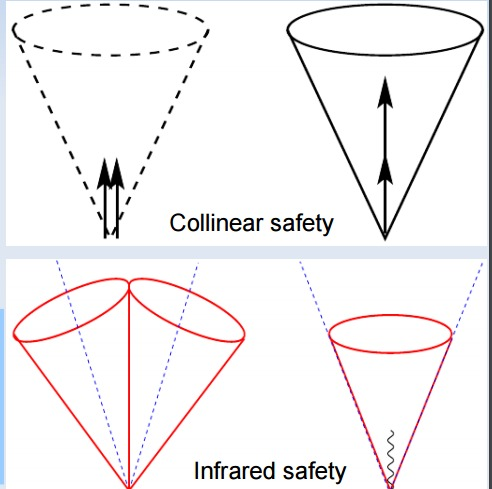
\includegraphics[width=3cm]{safe}
\end{wrapfigure}
Eşyönlü güvenilirlikte çıkan bir partonun yanında neredeyse aynı yönde $\theta = 0$ olacak şekilde başkabir parçacığa bozunuyorsa orada sonsuzluk veriyor ve bu jet yapılandırma algoritmasını bozuyor. Buna eşyönlü güvenilirlik deniliyor. 
Infrared güvenilirlik ise enerjisi çok düşük bir parçacık çıkıyorsa bu yine sonsuzluk meydana getiriyor buna buda tekrardan Jet yapılandırma algoritmasını bozmaktadır. Bu yüzden Jet yapılandırma algoritması hem eşyönlü güvenilir hemde Infrared güvenilir olması gerekmektedir.\\

